%%%%%%%%%%%%%%%%%%%%%%%%%%%%%%%%%%%%%%%%%
% FRI Data Science_report LaTeX Template
% Version 1.0 (28/1/2020)
% 
% Jure Demšar (jure.demsar@fri.uni-lj.si)
%
% Based on MicromouseSymp article template by:
% Mathias Legrand (legrand.mathias@gmail.com) 
% With extensive modifications by:
% Antonio Valente (antonio.luis.valente@gmail.com)
%
% License:
% CC BY-NC-SA 3.0 (http://creativecommons.org/licenses/by-nc-sa/3.0/)
%
%%%%%%%%%%%%%%%%%%%%%%%%%%%%%%%%%%%%%%%%%


%----------------------------------------------------------------------------------------
%	PACKAGES AND OTHER DOCUMENT CONFIGURATIONS
%----------------------------------------------------------------------------------------
\documentclass[fleqn,moreauthors,10pt]{ds_report}
\usepackage[english]{babel}
\usepackage{tcolorbox}
\usepackage{etoolbox}
\usepackage{todonotes}
\usepackage{numprint}
\usepackage{float}
\usepackage{cleveref}

\setuptodonotes{inline,backgroundcolor=yellow}

\graphicspath{{fig/}}




%----------------------------------------------------------------------------------------
%	ARTICLE INFORMATION
%----------------------------------------------------------------------------------------

% Header
\JournalInfo{FRI Natural language processing course 2024}

% Interim or final report
\Archive{Project report} 
%\Archive{Final report} 

% Article title
\PaperTitle{\textcolor{red}{WIP}: Literary Conversational Agents}

% Authors (student competitors) and their info
\Authors{Žiga Trček, Matej Urbas, and Jan Vasiljević}

% Advisors
\affiliation{\textit{Advisors: Slavko Žitnik}}

% Keywords
\Keywords{\textcolor{red}{DRAFT}, conversational agents, large language models, in-context-learning}
\newcommand{\keywordname}{Keywords}


%----------------------------------------------------------------------------------------
%	ABSTRACT
%----------------------------------------------------------------------------------------

\Abstract{
\textcolor{red}{DRAFT:} Engaging audiences deeply with literature is crucial for enhancing global literacy levels. In this study, we build upon the foundation of conversational agents, which have historically underperformed but have recently been revolutionized by advancements in large-scale language models. We fine-tune various foundational models and assess their enhanced capabilities using a series of standardized quizzes that we introduce. Our focus is on popular literary series, specifically "A Song of Ice and Fire" and "Harry Potter." Additionally, we underscore the significance of employing In-Context Learning to effectively emulate the dialogue styles of key characters within these series, thereby enriching the interactive reading experience.
}

%----------------------------------------------------------------------------------------

\begin{document}

% Makes all text pages the same height
\flushbottom

% Print the title and abstract box
\maketitle

% Removes page numbering from the first page
\thispagestyle{empty}

%----------------------------------------------------------------------------------------
%	ARTICLE CONTENTS
%----------------------------------------------------------------------------------------

\section*{Introduction}

Literacy among young people is declining, as highlighted in \cite{murray2021literacy}. Many young people have a disinterest in reading and seldom read for enjoyment. A potential strategy to encourage reading is to involve them in conversational interactions with digital pedagogical agents that imitate well-known literary figures. Although numerous studies, such as those \cite{nielen2018digital,alaimi2020pedagogical}, discuss the advantages of pedagogical agents, detailed technical implementation aspects are often overlooked. Our work aims to explore various methods for creating pedagogical agents and to provide a comprehensive technical implementation for the method we choose.

\subsection*{Related work}
In \cite{papaioannou2022designing} they built a social bot, called Alana, which is able to engage in an open-domain conversation with their users over various popular topics. The key requirements for such a bot are to maintain the context, provide coherent responses, and be engaging and knowledgeable. The final bot is an ensemble of many different bots, each of which has a different purpose. A ranker is used to determine the best bot response for the given user input. For context maintaining, a state object with information from previous conversations is stored and accessible to every bot in the ensemble.

Retrieval augmented generation (RAG) is often used to correct factually inaccurate, outdated or halucinated Large Language Model (LLM) outputs. A survey on different RAG methods is conducted in \cite{gao2023retrieval}. RAGs can be seprated into three categories: pre-training, fine-tunning and inference. Nowdays inference RAGs are mostly used. \cite{jiang2023active} proposed FLARE, Forward-Looking Active REtrieval Augmented Generation, which re-prompts the language model with extra retrieved data about the subject when some tokens in LLM's output have a low probability.

A straightforward way to create agents is by training or fine-tuning LLM. In \cite{shao2023characterllm} the authors developed conversational agents that resemble historical figures like Beethoven, Cleopatra, and Caesar, with personalized profiles, experiences, and emotional states. They introduced three new methods for training specialized agents. Experience Reconstruction extracts scenes in the style of memory flashes, such as profiles, scenes, or interactions. Protective Experience aims at teaching the model to forget or ignore information not relevant to the character to prevent knowledge hallucinations. Experience Upload uses the previous two techniques to fine-tune an existing LLM. They fine-tuned a LLaMa 7B model \cite{touvron2023llama} on a dataset of \numprint{750000} words per character using eight A100 80GB GPUs for 1 hour per character. To assess the models, they used an interview process.

Obtaining data to train a character can be difficult.
\cite{neuman2023data} proposes a novel data augmentation approach named PEDANT that helps train models that mimic human personality by generating large amounts of data with a GPT combined with domain expertise.
The method first gathers unlabeled data from online resources and trains a generative language model with it.
Then, this model is prompted with seed sentences that an expert created and is asked to complete them.
Then, these completions are filtered and ranked based on an expert-defined scoring function.
In the paper, PEDANT was implemented on an anti-social psychopatic personality disorder.
A labeled corpus with this disorder does not exist, so this is a good showcase of the usefulness of the approach.
The data to train the GPT comes from cinema, TV, and Reddit.
The model was validated using a text classification task.
They used the generated data to train a classifier and tested it on offensive-speech datasets.
The results were very encouraging, but requires domain knowledge, which can be a big limiting factor and bottleneck in a larger process.

To avoid training a LLM, \cite{jeong2023chatbot} suggests using prompt engineering, specifically Chain-of-Thought (COT), on an existing model to incorporate more contextual information. They recommend employing Information-Rich Prompts (IRP) that include the emotional state, the character's relationship with the interlocutor, and the character's memories. Memories are categorized into short-term, which are a limited number of the most recent conversations with the interlocutor, and long-term, which are recursively summarized memories of longer conversations from the character's perspective. Although not explicitly stated, implementing the Big Five personality model \cite{goldberg1990thebigfive} could further refine the character's responses. This model would detail the character's Openness, Conscientiousness, Extraversion, Agreeableness, and Neuroticism.

Previous methods that do not involve fine-tuning could be enhanced by using the OpenICL framework \cite{wu2023openicl}. In-Context Learning (ICL) is an approach used with LLMs where the model learns a specific task without the need to update its weights. Instead, the model is shown examples of how the task should be performed. OpenICL offers the tools needed to construct ICL tasks, including key components like retrieval strategies and inference methods. For retrieval, it incorporates heuristic-based methods (such as BM25 and Top-K), random sampling, and model-based retrieval (using embeddings, RAG, Minimum Description Length (MDL), and entropy-based selection). For inference, OpenICL facilitates the integration of COT and other methods along with a prompt template.

It is important to consider teaching strategies while implementing an agent that serves an educational purpose.
\cite{bogaerds2022textbooks} carried out a detailed analysis of reading comprehension textbooks from the Netherlands, which is one of the nations with a low comprehensive literacy.
The researchers analysed lessons withing the textbooks and then also analysed the utilisation of these textbooks by teachers, both by conducting interviews with teachers and attending live lessons.
They found that the lessons are mostly focused on exercising and that there is no strong alignment between goals of the lessons, the theory behind them and the assignments that the students must carry out.
Little actual knowledge about reading strategies was illustrated and there was no opportunity to choose and apply strategies yourself.
The interviews showed that the teachers were aware of these problems, but there were very few who adapted the lessons to counteract them and improve the quality of their teaching.
The knowledge that was observed in the textbooks was divided into:
\begin{itemize}
	\itemsep0em
	\item declarative knowledge - knowing something
	\item procedural knowledge - knowing how to do something
	\item conditional knowledge - knowing when to do something.
\end{itemize}
The textbooks were mostly just focused on the procedural part of the knowledge.
To improve literacy, all three should be taught.

\cite{situation_models} describes the importance of setting and situational continuity while reading, which can have major implications in providing a good user experience.
Three experiments were carried out on 27 psychology students that tested which aspects of a five-dimensional situational model are more important to our experience.
They tested the impact of different aspects by measuring reading time while introducing discontinuities across different dimensions (time, space, causation, motivation, protagonist).
The reading time increase is very noticeable in all but the spatial dimension.
There, spatial discontinuities did not present a large increase in reading time unless the study participants memorized the map of the story space in advance.
The study confirmed the "processing-load hypothesis" that predicts that the reading time goes up when there is more data to process.
It's very likely that this information could be taken into account when constructing a model used for learning by keeping continuities along dimensions that are irrelevant for the learning experience and channeling the focus elsewhere.


BookNLP \cite{booknlp} is a NLP pipeline that supports the analysis of literary texts. It does POS tagging, dependancy parsing, entity recognition with co-reference resolution and clustering, event tagging and more. It's built on top of Spacy \cite{spacy2} and uses BERT \cite{joshi2019bert} for co-reference resolution. It provided a good pipeline for extracting dialogues from the books and attributing them to characters.

%------------------------------------------------

\section*{Methods}


\todo[author=Jan]{
	\textbf{To smo pisal pred 2. zagovorom. Ne vem a se pustimo ali drugace oblikujemo.}

	We used \cite{touvron2023llama} and \cite{abdin2024phi} as our base models.
	We fine-tuned them on a preprocessed full-text dataset from Harry Potter novels.
	We trained the models using overlapping chunks of text to ensure that the model learns the context of the conversation.
	We used a chunk size of 512 characters and an overlap of 64 characters.

	In the future, we will extract all dialogues from the Harry Potter and A Song of Ice and Fire series and use them to fine-tune the models.
	This will allow the models to have contextual knowledge to provide a more accurate depiction of characters.
	We aim to construct a dataset of quotes from the literary works and the characters who said them.
}

\subsection*{Data}


\subsubsection*{Dialogue Extraction Using Instruct LLM}

We extracted all the dialogue along with the pre and post context (10 sentences before and 2 after each dialogue) and used Phi3 and Llama8B to classify the dialogue by identifying the speaker. We ignored dialogues shorter than 16 characters (not meaningful) and longer than 500 characters (to save VRAM consumption). With a batch size of 10 dialogues, we classified all \numprint{40318} dialogues in 7 hours. We used a 2 and 4-shot prompt with examples of classification but didn't achieve good results. There were three main reasons for this:

\begin{enumerate}
	\item The models didn't possess good enough reasoning capabilities to classify the dialogues.
	\item Co-reference resolution was not good enough to classify the dialogues. When pronouns were used, the model didn't know who was speaking most of the time.
	\item Information leakage: The models clearly had some prior knowledge about the books, as they sometimes classified the dialogue with characters that weren't even present in the pre or post context or the dialogue itself.
\end{enumerate}

By validating the data by hand, we realized we wouldn't get good enough results with this approach.


\subsubsection*{Dialogue Extraction Using BookNLP}

We used BookNLP to extract dialogues from both books. The \texttt{big} model provided by the authors of BookNLP was utilized, which required 5-8 minutes of processing time per book. We also attempted to merge the books before processing to improve co-reference clustering and resolution; however, this resulted in memory segmentation faults, even on a machine with 128GB of RAM (Arnes). Consequently, we processed each book individually, necessitating the correct correlation of character names across the series. This process involved normalizing names and removing duplicates by extracting sub-tokens and taking the root with the highest occurrence. If two sub-tokens had the same occurrence, we joined them, indicating a name with a space in it. For example, the character \textit{Hot Pie} from the series "A Song of Ice and Fire."

To validate the results, we manually reviewed randomly sampled dialogues. Based on this assessment, we assesed that approximately 90\% of the dialogues were correctly classified. Additionally, we constructed two graphs that show the dialogue frequency by character per book in the series (\cref{fig:asoif_dialogue} and \cref{fig:hp_dialogue}). Based on our familiarity with the books, we can confirm that the results are accurate. In the "A Song of Ice and Fire" series, the chapters are also told from the perspective of the characters, so we matched the frequencies with their respective chapters. In total, we gathered \numprint{36946} dialogues from ASOIAF and \numprint{32541} from HP, totaling \numprint{69487} dialogues.

\begin{figure}[H]

	\centering
	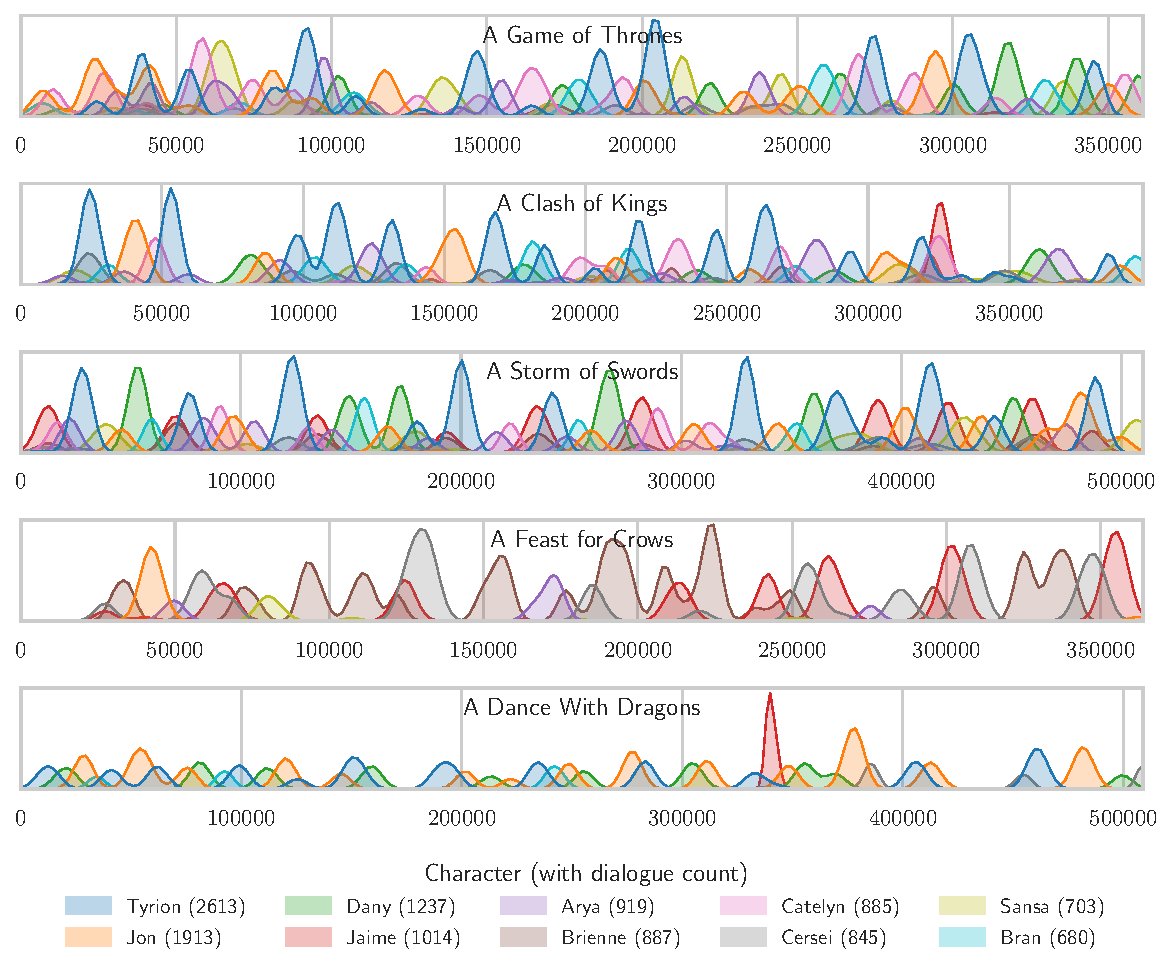
\includegraphics[width=\linewidth]{asoif_dialogue.pdf}
	\caption{\textbf{Dialogue from 10 most frequent characters in A Song of Ice and Fire.} This shows the dialogue frquency by character per book in the serioes. The x-axis represents the token count when the character speaks, while the y-axis the kernel density estimate of the dialogue frequency.}
	\label{fig:asoif_dialogue}
\end{figure}


\begin{figure}[H]

	\centering
	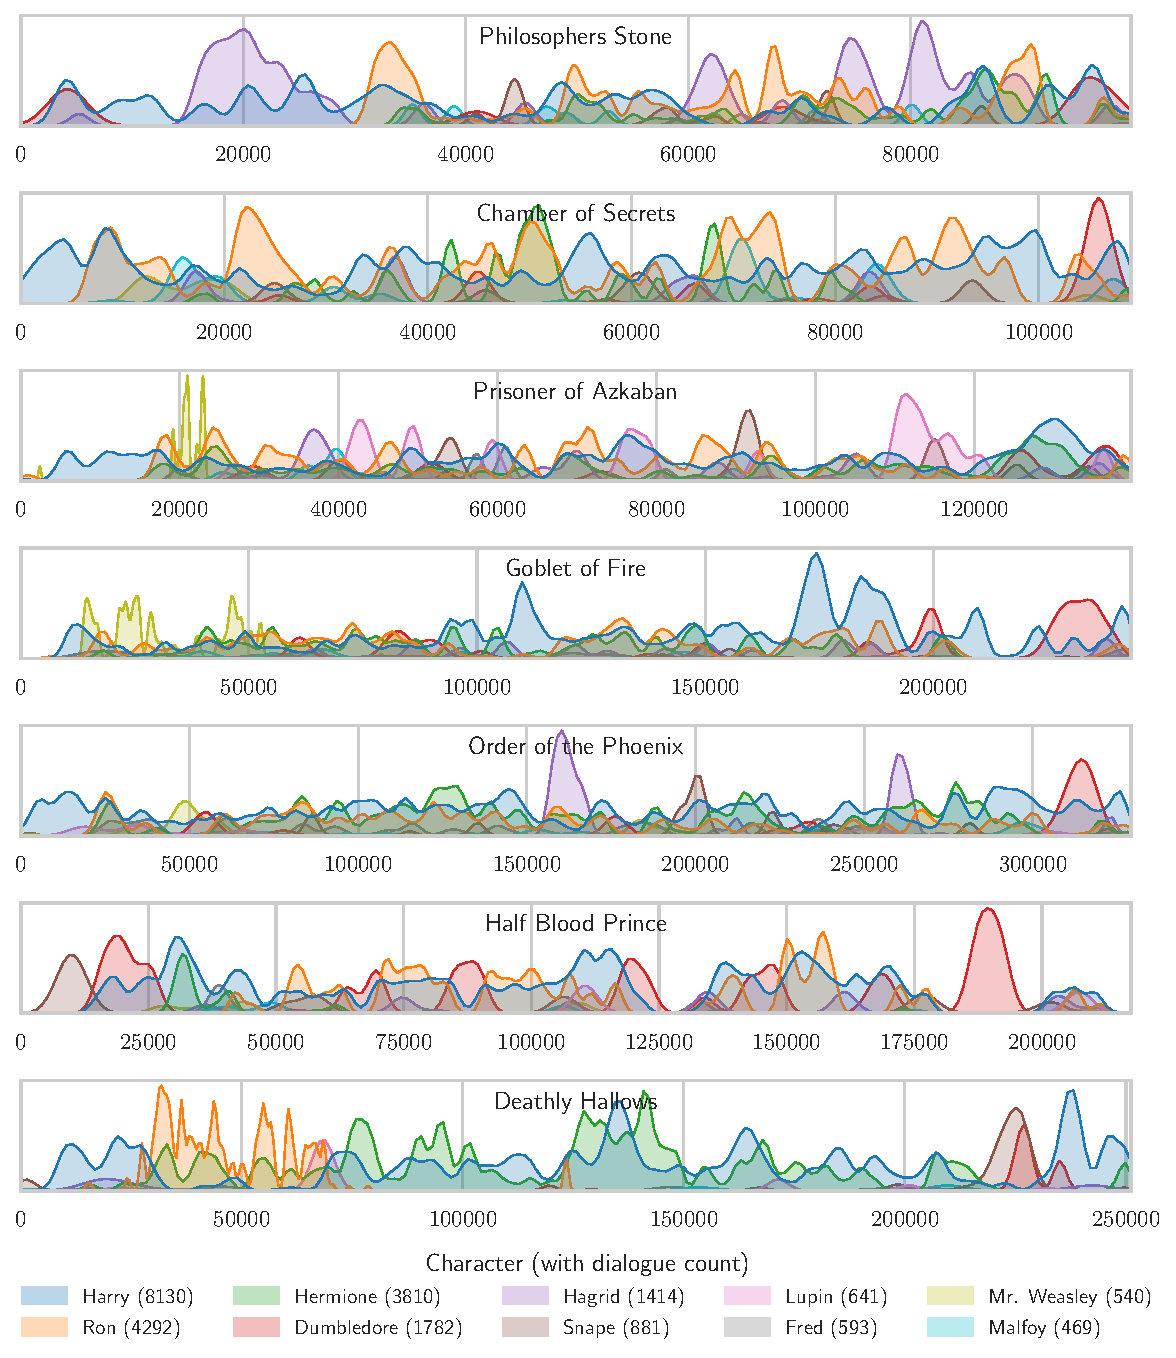
\includegraphics[width=\linewidth]{hp_dialogue.pdf}
	\caption{\textbf{Dialogue from 10 most frequent characters in the Harry Potter series.} This shows the dialogue frquency by character per book in the serioes. The x-axis represents the token count when the character speaks, while the y-axis the kernel density estimate of the dialogue frequency.}
	\label{fig:hp_dialogue}
\end{figure}




\subsubsection*{Other unsuscsessful attempts}

After extracting dialogues, we attempted several other methods to extract data from the books. The goal was to enhance the conversational model by providing it with more context from the books. These methods included:

\begin{enumerate}
	\item Extracting factual information from the books by re-using named entity recognition (NER) entities related to the characters. We extracted subject-verb-object triples from the books to gain more information about the characters. However, due to the complexity of the language used in the books, the extraction did not yield meaningful results.

	\item  \todo{Tole sm pol naredu, mogoče spremeni, da si probal dobit neke lastnosti characterjeu?} Recursively summarizing the books to achieve a better understanding of the characters and their relationships. We used Phi3 with a 128k context window to recursively summarize sections of the books that included a particular character of interest. This approach, however, did not succeed. It was computationally expensive (even after splitting into 20k chunks, the model used upwards of 60GB of graphics memory) and the results were inadequate. Despite claims that the model can handle tasks within a long context, the results showed that the model completely forgot the instructions after utilizing only 1/8 of its theoretical context window.

	\item Using DistilBART for question answering. Our final attempt was to extract key information about characters from the books (such as character locations, ages, etc.) and use DistilBART to answer questions. This was intended to serve as in-context learning for our conversational agents. However, this approach also failed due to the complex language used in the books.

\end{enumerate}

\subsection*{Book summaries}
The characters' dialogues can give the language model an idea about how a specific character speaks; however, it can still use more context to formulate a better answer.
Furthermore, many of the important contextual information can't be extracted from speech alone.
By giving the langauge model extra content from the books we hoped to increase its performance in some evaluation tasks.

Original texts are quite long. A Song of Ice and Fire consist of around 1.7 million words. The Harry Potter series is a bit shorter with 1.1 million words. Therefore we split the books into smaller chunks and summarized each of them. We tried a few different summarization language models from HuggingFace:
\todo[]{Citirat modele?}
\begin{itemize}
	\item bart-large-cnn
	\item google-t5/t5-large
	\item google/pegasus-xsum
	\item Falconsai/text\_summarization
\end{itemize}

By examining the outputs we concluded that the Falconsai's model gives the best summarizations.
It has a context window of 512 tokens, therefore we split the books into chunks, smaller than 512 tokens.
Splitting was done only between sentences so they were never cut in half, which resulted in chunks being smaller than 512 tokens.
This gave us 6275 chunks from A song of Ice and Fire and 4716 chunks from the Harry Potter series.
Summarization of all 10991 chunks took about 6 hours and resulted in around 6 fold word count reduction. Summarized Song of Ice and Fire consists of around 300k, and Harry Potter series of around 200k words.

\subsection*{Retrieval augmented generation}
We stored the selected character's dialogues, with or without surrounding context, in a FAISS vector database.
During inference the database was queried by the user's question and returned between 10 and 30 promising character lines,
which were then used to create the model prompt.
Same was done with book summaries to provide the model with some additional context.

\subsection*{Figures}

On the other hand, \figurename~\ref{fig:whole} is an example of a figure that spans across the whole page (across both columns) of the report.

% \begin{figure*} makes the figure take up the entire width of the page
\begin{figure*}[ht]\centering
	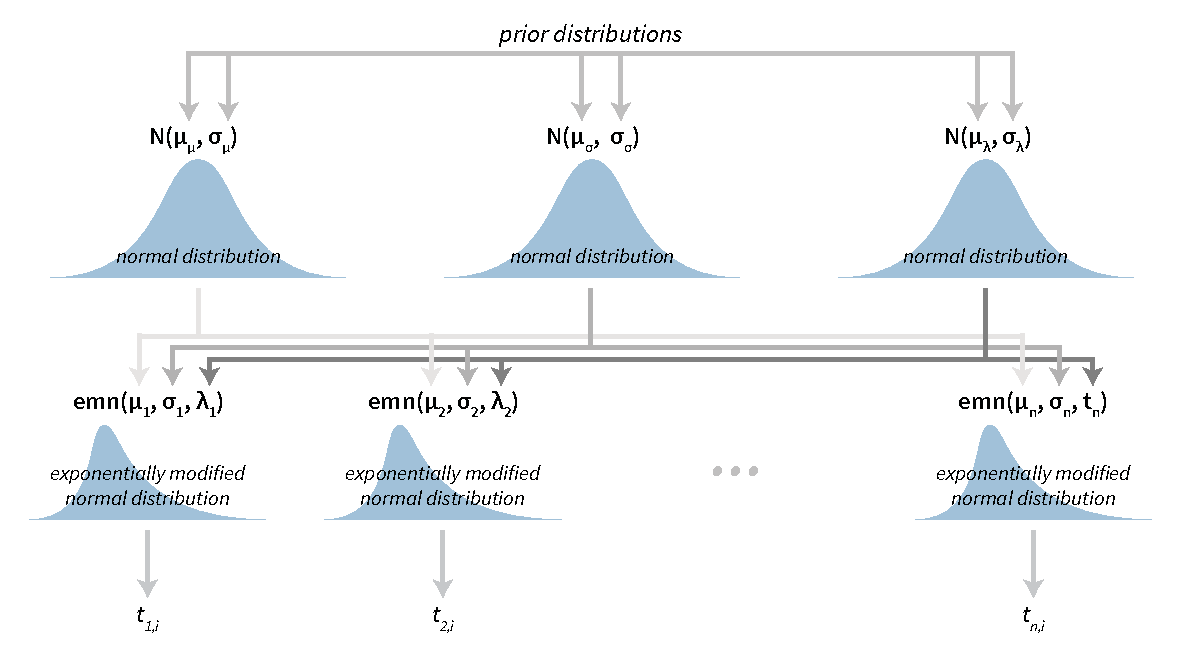
\includegraphics[width=\linewidth]{whole_page.pdf}
	\caption{\textbf{Visualization of a Bayesian hierarchical model.} This is an example of a figure that spans the whole width of the report.}
	\label{fig:whole}
\end{figure*}


\subsection*{Tables}

Use the table environment to insert tables.

\begin{table}[hbt]
	\caption{Table of grades.}
	\centering
	\begin{tabular}{l l | r}
		\toprule
		\multicolumn{2}{c}{Name}       \\
		\cmidrule(r){1-2}
		First name & Last Name & Grade \\
		\midrule
		John       & Doe       & $7.5$ \\
		Jane       & Doe       & $10$  \\
		Mike       & Smith     & $8$   \\
		\bottomrule
	\end{tabular}
	\label{tab:label}
\end{table}


\subsection*{Code examples}

You can also insert short code examples. You can specify them manually, or insert a whole file with code. Please avoid inserting long code snippets, advisors will have access to your repositories and can take a look at your code there. If necessary, you can use this technique to insert code (or pseudo code) of short algorithms that are crucial for the understanding of the manuscript.

\lstset{language=Python}
\lstset{caption={Insert code directly from a file.}}
\lstset{label={lst:code_file}}
\lstinputlisting[language=Python]{code/example.py}

\lstset{language=R}
\lstset{caption={Write the code you want to insert.}}
\lstset{label={lst:code_direct}}
\begin{lstlisting}
import(dplyr)
import(ggplot)

ggplot(diamonds,
	   aes(x=carat, y=price, color=cut)) +
  geom_point() +
  geom_smooth()
\end{lstlisting}

%------------------------------------------------

\section*{Results}

\todo{This was for 2nd submission}

We evaluated our fine-tuned models on a dataset of 108 multiple-choice quiz questions about the Harry Potter series.
The questions were designed to test the models' understanding of the characters and their relationships.
The models achieved an average accuracy of 72\% before and after fine-tuning.

We also evaluated the models with a sorting hat quiz, where the model had to solve a quiz as a character from a given house (Gryffindor, Hufflepuff, Ravenclaw, or Slytherin).
The models were always classified into Ravenclaw.

We plan to evaluate the models on a dataset of quiz questions about the A Song of Ice and Fire series.

We will also evaluate our models on state of the art benchmarks, as in \cite{guo2023evaluating}.
Use the results section to present the final results of your work. Present the results in a objective and scientific fashion. Use visualisations to convey your results in a clear and efficient manner. When comparing results between various techniques use appropriate statistical methodology.

\todo{Here starts the "final" evaluation}
Most of the evaluation was manual, therefore slightly subjective.
It was done independently by all three team members and averaged into the final conclusion.

\subsection*{Character evaluation}
We looked at the language model's ability to speak as a selected character.
For this test we picked 6 characters, 3 from both series.
From the Harry Potter franchise we picked Harry Potter himself, headmaster Dumbledore and antagonist Voldemort.
For A Song of Ice and Fire we picked mother of dragons Daenerys, lord commander John Snow and the best door holder Hodor.

We created a list of questions for every character.
There are 8 non-specific questions (for all 6 characters), 9 Harry Potter specific questions, 14 ASOIF specific questions
and for each character an additional 4-8 questions.
In total there are 30 different questions for Harry Potter and 40 questions for ASOIF characters.

The biggest evaluation problem was quite unexpected. It was very difficult to find an appropriate large language model for this task.
Bigger language models, such as Llama-3-8B \cite{llama3modelcard} or Mistral-7B \cite{jiang2023mistral} were already so familiarized with both series that the model worked good without any modifications.
Smaller language models, such as TinyLlama-1.1B \cite{zhang2024tinyllama}, GPT2 \cite{radford2019language} or Google Gemma-2B \cite{gemma_2024},
were either unable to act as a given character (saying that they are a langauge model and unable to answer the question)
or their answers were very random, and not connected to the books in any way, despite trying several different prompts and RAG strategies.
In the end we decided to use Microsoft's Phi-3 \cite{abdin2024phi} and Phi-2 models, pretrained for instruction tasks.
These two models weren't as familiar with the characters but were still able to somewhat act as the desired character.

For each character we tested three different prompting strategies:
\begin{itemize}
	\item Prompt contained only the name of the character and the book series and some instructions how to act. This was done so that we can get a rough baseline of what the model knows and how it behaves out of the box.
	\item This prompt extended the previous one with dialogues and other context retrieved from the vector database.
	\item This prompt didn't state the character name or the book series. Only data that the model recieved was retireved from the vector database.
\end{itemize}

Each of the two models answered 150 questions across all characters using all three prompting strategies, which resulted in 900 total answers.
For every member in the group we randomly sampled 60 answers from Harry Potter and 60 from A Song of Ice and Fire.
Half of the questions were answered by Phi-2 and the other half with Phi-3.
Answers were randomly mixed, so that we didn't know which prompting strategy resulted in which answer.
We then ranked the answers from best to worst based on the overall structure, answer quality and information correctness.
In total we checked 360 questions with 1080 answers.
For each prompting strategy we summed its final ranks and sorted them accordingly.
Final rankings are shown in Tables \todo[]{Dodaj grafe etc}

\subsection*{Sorting hat test}
We thought it would be interesting to evaluate our Harry Potter characters with the sorting hat test.
This evaluation was done out of curiosity. The rules of the sorting test are not really stated inside the book.
We scraped a random online sorting hat quiz which looked promising and easy to use.
We used the quiz on 8 different characters, 2 from each house:
\begin{itemize}
	\item Gryffindor: Harry and Dumbledore,
	\item Slytherin: Snape and Draco,
	\item Ravenclaw: Cho and Luna,
	\item Hufflepuff: Cedric and Tonks.
\end{itemize}
Each character was tested with all three prompting strategies, with Phi-3 as the language model.
We ran the test 10 times for every character.
The test results are shown in Table \ref*{tab:sorting_hat_results}. Correct house predictions are in bold.

\begin{table}[hbt]
	\caption{Sorting hat results}
	\centering
	\begin{tabular}{c | c | c | c }
		Character  & Without RAG        & RAG hidden          & RAG reveal          \\ \hline
		Harry      & Slytherin          & \textbf{Gryffindor} & \textbf{Gryffindor} \\
		Dumbledore & Slytherin          & \textbf{Gryffindor} & \textbf{Gryffindor} \\ \hline
		Snape      & \textbf{Slytherin} & Gryffindor          & \textbf{Slytherin}  \\
		Draco      & \textbf{Slytherin} & Gryffindor          & \textbf{Slytherin}  \\ \hline
		Cho        & \textbf{Ravenclaw} & Gryffindor          & \textbf{Ravenclaw}  \\
		Luna       & \textbf{Ravenclaw} & Gryffindor          & \textbf{Ravenclaw}  \\ \hline
		Cedric     & Slytherin          & Gryffindor          & Ravenclaw           \\
		Tonks      & Gryffindor         & Gryffindor          & Gryffindor          \\
	\end{tabular}
	\label{tab:sorting_hat_results}
\end{table}

%------------------------------------------------

\section*{Discussion}

Our fine-tuning attempts have not been successful so far.
The baseline models perform well on the quiz questions and simple fine-tuning does not seem to improve the performance.
We will try to extract more context from the books using more sophisticated approaches and use it to fine-tune the models.

The dialogue generation is also very good out of the box, especially with smart prompting.
We will try to improve the dialogue generation by using context databases.


\todo{After the 1st phase}

Use the Discussion section to objectively evaluate your work, do not just put praise on everything you did, be critical and exposes flaws and weaknesses of your solution. You can also explain what you would do differently if you would be able to start again and what upgrades could be done on the project in the future.


%------------------------------------------------

\section*{Acknowledgments}

\todo{After the 1st phase}

Here you can thank other persons (advisors, colleagues ...) that contributed to the successful completion of your project.


%----------------------------------------------------------------------------------------
%	REFERENCE LIST
%----------------------------------------------------------------------------------------
\bibliographystyle{unsrt}
\bibliography{report}


\end{document}
